\section{Redshift distribution}
Redshift distribution of LRGs is constructed from the DESI SV data release of Denali with the same selection. The fiducial distribution only covers the redshift range from 0.2 to 1.35. Below we test the impact of LRG dN/dz on the angular power spectrum.


\begin{figure}
\centering
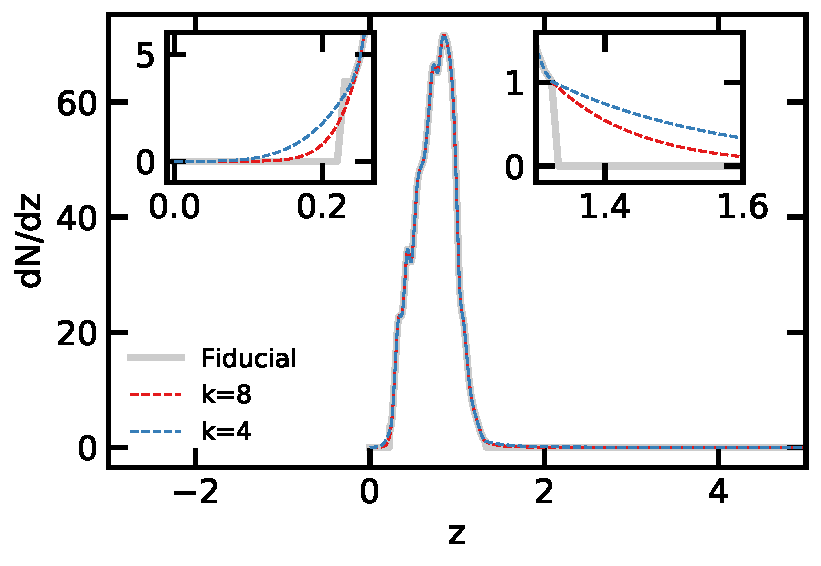
\includegraphics[width=0.45\textwidth]{nztreat.pdf}
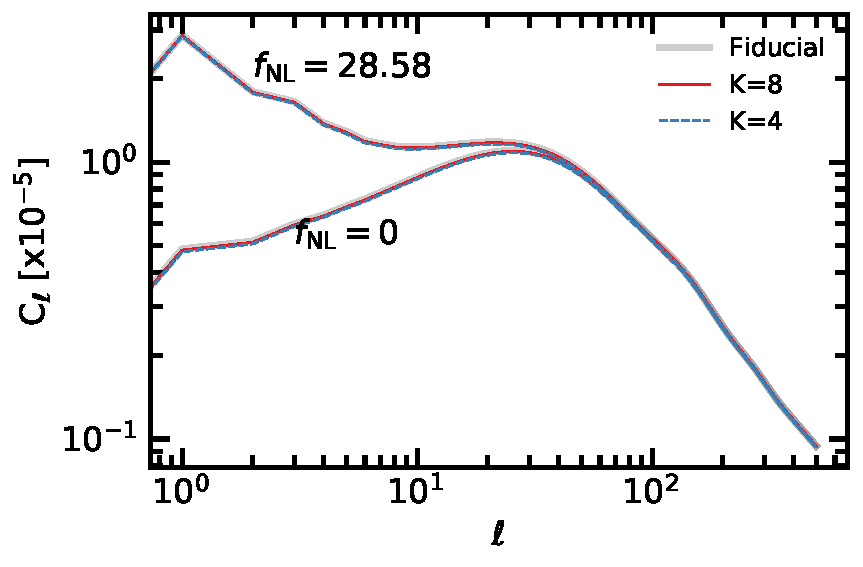
\includegraphics[width=0.45\textwidth]{cell_nz.pdf}
\caption{Top: Redshift distribution of LRGs. Bottom: Power spectrum given various dN/dz treatments for two arbitrary $\fnl$ values.}
\end{figure}


\section{Scale dependence systematics}
The default modes used in calculating the cross spectrum $\chi^{2}$ diagnostic range for $2 \leq \ell < 20$. Here we further test the stability of our results by extending the highest mode out to $\ell=100$ or fluctuations over scales as small as $1.8$ degrees. 
\begin{figure}
\centering
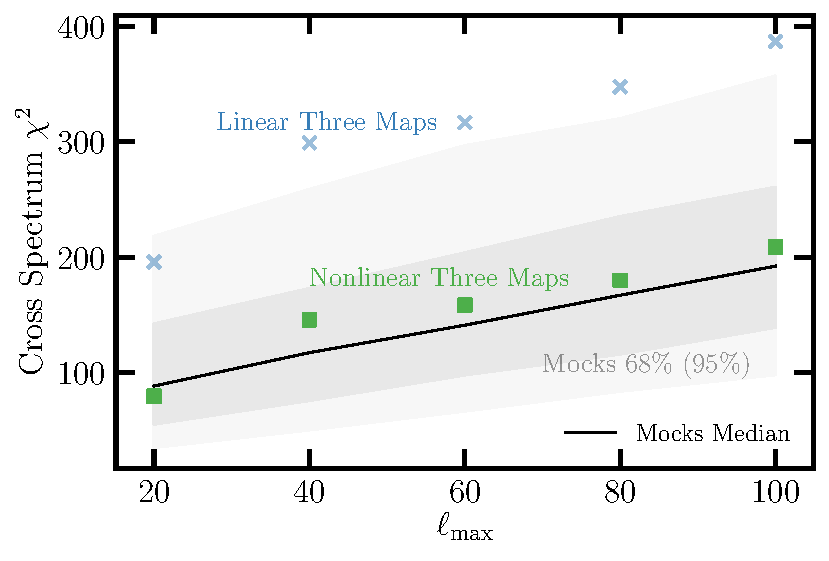
\includegraphics[width=0.45\textwidth]{chi2lmax.pdf}
\caption{Cross Spectrum $\chi^{2}$ as a function of the highest mode $\ell_{\rm max}$. The lowest mode is $\ell_{\rm min}=2$.}
\end{figure}